\documentclass{article}
\usepackage[margin=1in]{geometry}
\parindent=0in
\parskip=8pt
\usepackage{graphicx}
\usepackage{parskip}

\begin{document}

\section{Doug Healy}

I am starting my second year in work towards my PhD in Engineering Security, studying under Dr. Bloom. I received my Masters in Information Security Policy and Management (MSISPM) from Carnegie Mellon in 2013, and my BS in Electrical Engineering Technology back in 2003 from the Rochester Institute of Technology (RIT). 

I am a avid and active supporter of Scouts BSA, volunteering much of my time in support of the program, both at the Scout (11 to 18 years old) and Cub Scout (5-11 years old) levels. Being an Eagle Scout myself, I highly believe in the values and qualities it instills in our young men and women and work very hard to make the programs successful and FUN!  

For this course, I hope to become more efficient in my research. I have spent many, many hours over the summer pouring over search results from both Google Scholar and the UCCS Library. I want to learn how to hone search results, use the correct resources, to efficiently find what I am actually looking for, not what some search engine "thinks" I am looking for. This will also require me to refine how I choose my search terms.  

Secondly, I want to learn how to effectively learn to use my time in reading a scholarly document. I am not a good "skimmer" of documents or books; never have been. I want to learn how to do this more effectively and to make sure I am not missing anything. I always think I am missing important things on the page, and I want to ensure that through my skimming, I am not.   

\subsection{My Picture: }
\begin{figure}[htp]
    \centering
    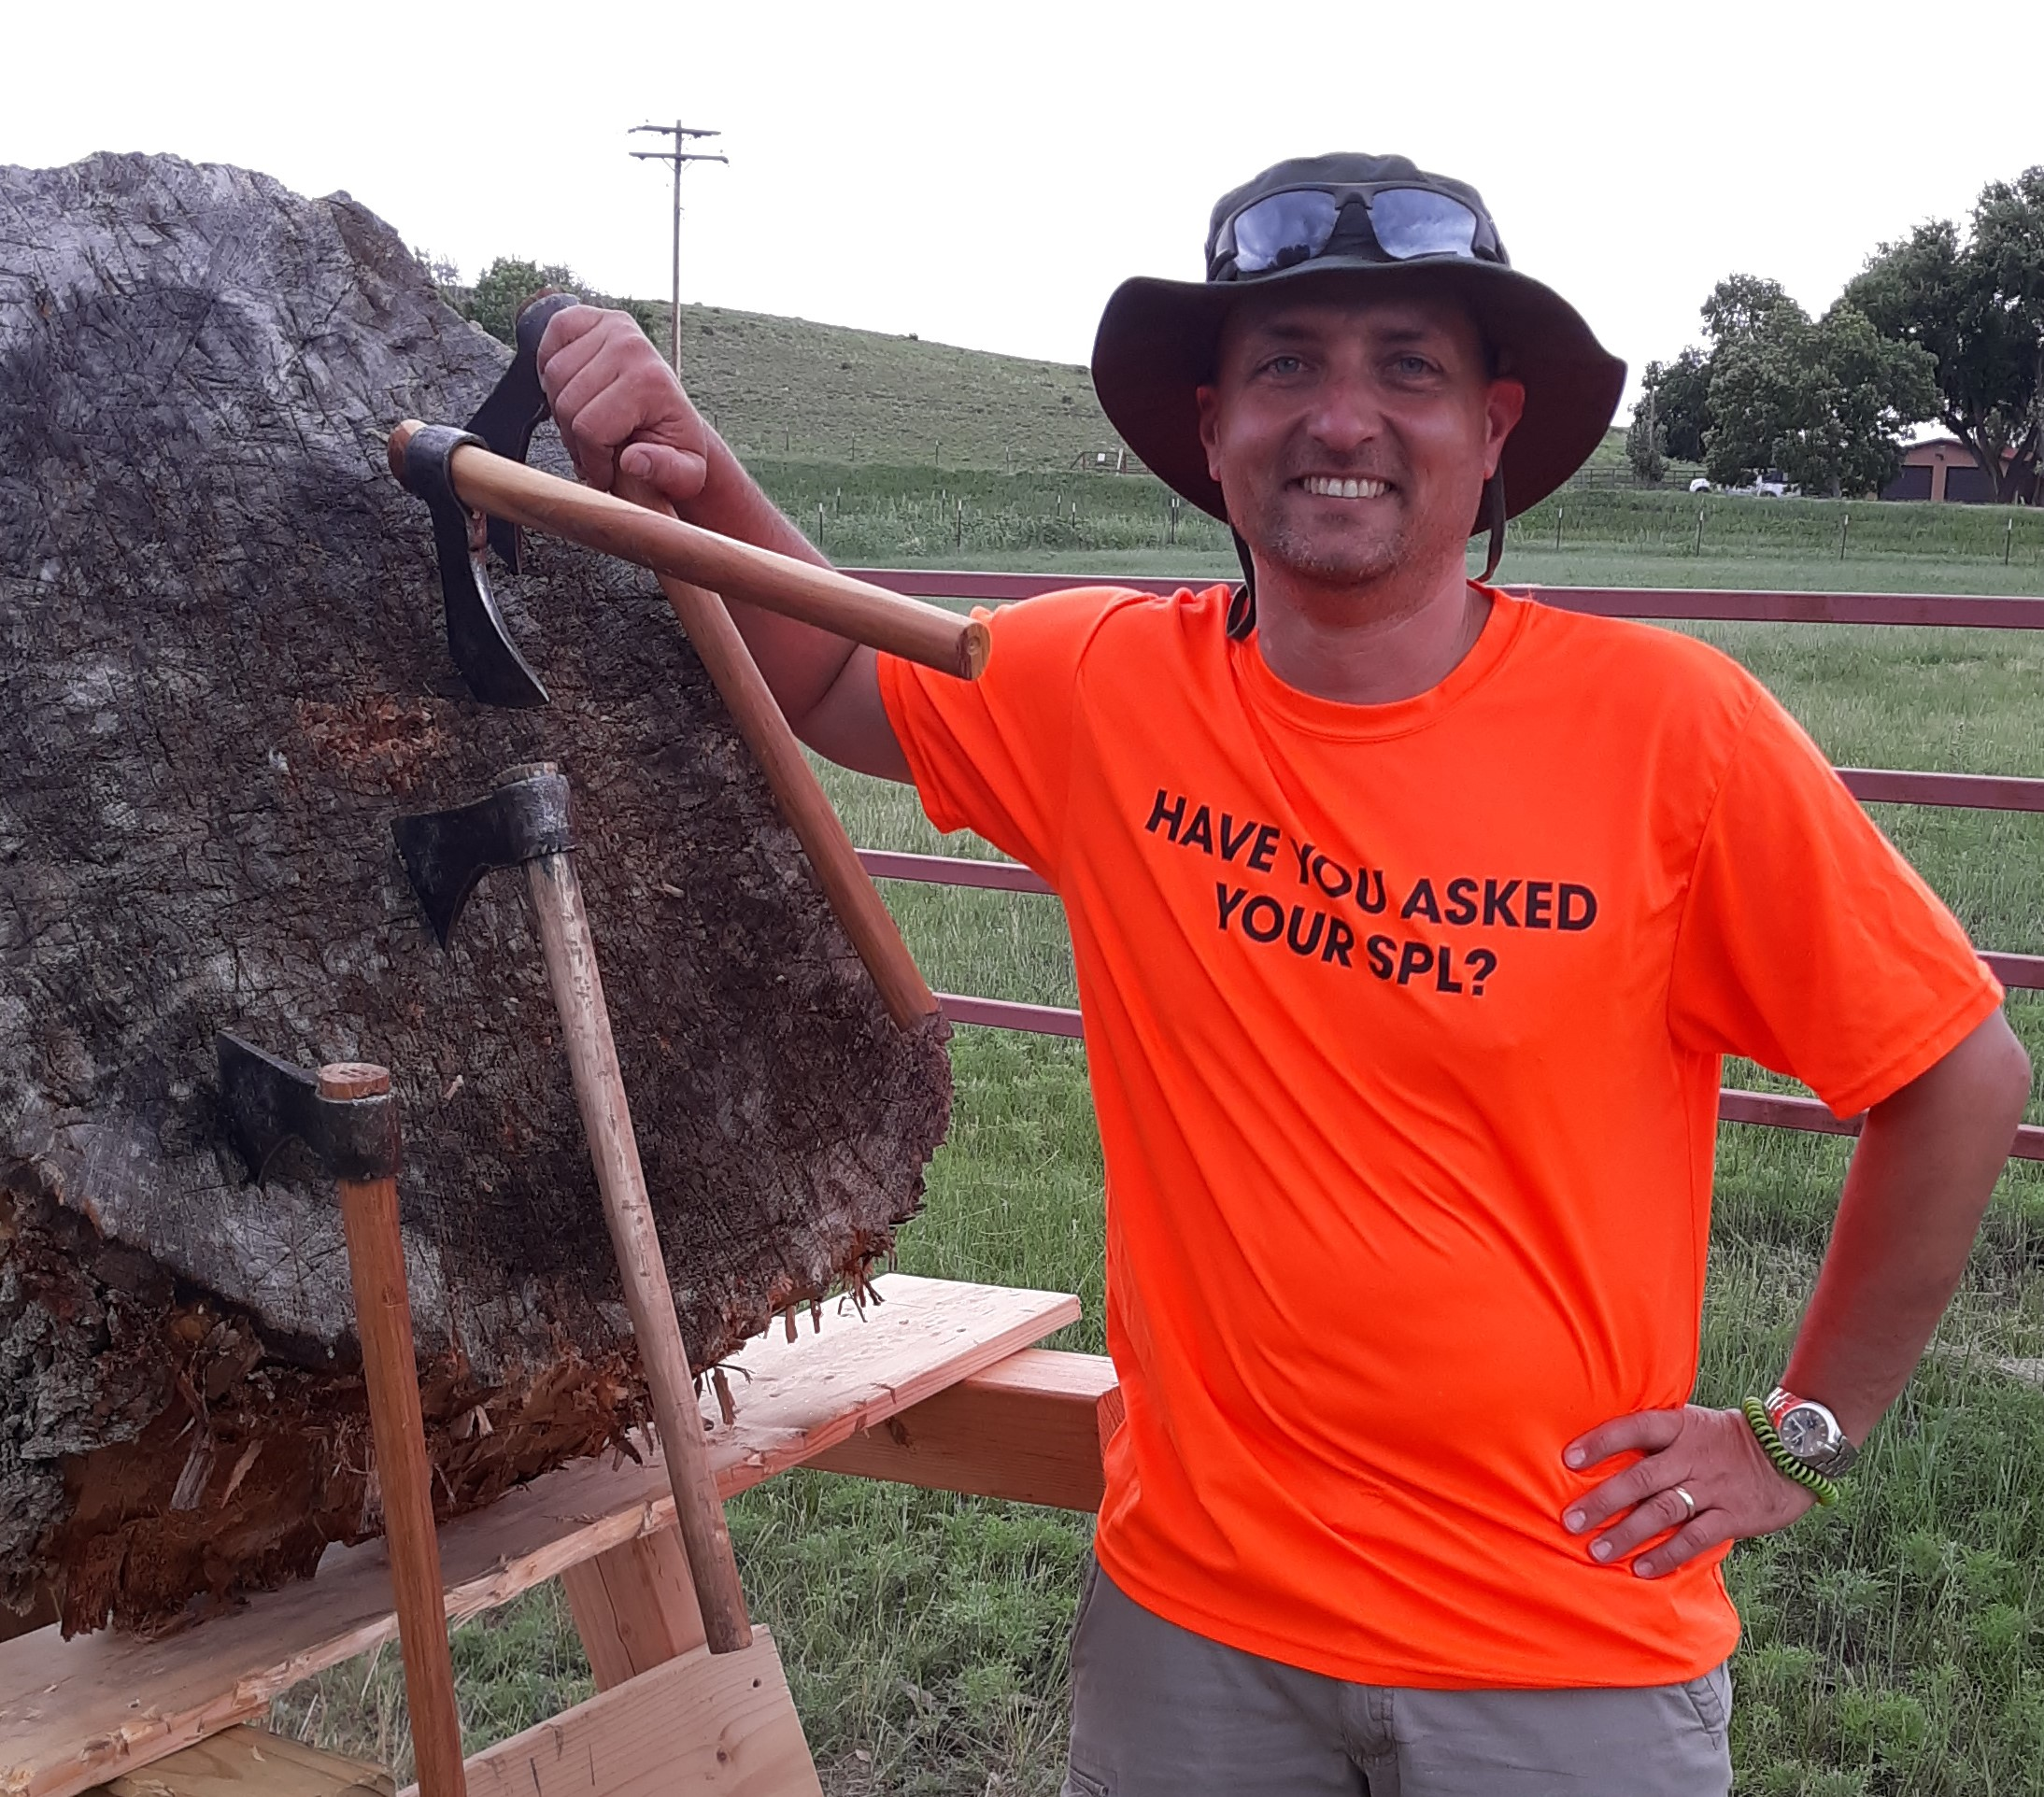
\includegraphics[scale=.095]{Healy.jpg}
    \caption{Doug Healy at Philmont Scout Ranch, Cimarron NM}
 \end{figure}
\end{document}
